\section{实验}
\label{sec:results}

\subsection{设置}
\label{sec:results_setup}

我们对比了得分中心化方法与 \Cref{tab:is_methods} 中的修正方法，在 \citep{stream_of_search} 上训练 Qwen3-0.6B-Instruct，以及在 {INTELLECT-2} 数据集的数学子集 \citep{intellect2} 上训练 Qwen3-30B-A3B-Base。

\noindent\textbf{共享目标.} 现有方法通常将多种技术组合在一起：例如，DAPO 将非对称裁剪与动态采样 \citep{dapo} 结合，而 IcePop 将训练与推理引擎之间的 MIS 与策略版本间的 PPO 裁剪 \citep{icepop} 结合。为了单独比较每种修正方法，我们全程使用相同的目标（以组中心奖励为基准的 REINFORCE），并将每种修正方法单独应用于该目标之上。所有方法共享相同的采样器、训练器、优化器和优势函数，每个批量执行一次 SGD 步骤。所有重要性比率均使用采样器记录的概率。\Cref{tab:is_methods} 展示了修正规则和超参数，以及实现说明。学习率、批量大小和计算成本列于 \Cref{sec:experimental_details}。

\noindent\textbf{不匹配情景。} 通常情况下，我们难以找到自然的设置，使得TIM严重到能够在数小时的GPU训练时间内观察到表现最强的方法之间的统计显著差异。我们认为这是训练过程中漂移累积的结果（\Cref{sec:sc}）：在轻微的TIM下，需要更多的训练步数才能积累足够的漂移，而在漂移足够之前，表现最好的方法会重叠。我们在 \Cref{sec:results_weight_noise} 中展示了这一点：在较小的权重噪声下，表现最好的方法重叠，导致无法进行比较；而随着TIM的增加，方法更早崩溃，它们之间的性能差距也逐渐增大。由于我们无法负担在极长训练周期中对校正方法进行具有统计显著性的消融实验，因此我们故意放大TIM，将这些结果作为在较温和TIM下大规模训练的代理。出于这一原因，在 \Cref{sec:results_quant_stale} 中我们测试了故意严重的量化和延迟设置。值得注意的是，先前的工作对于强化学习在TIM下的实际不稳定性存在分歧：\citet{fp8_rl} 发现仅使用token级重要性采样且不匹配数值的情况下，fp8回放仍保持稳定；而 \citet{mai_1} 在尽力最小化TIM并使用bf16采样时，仍观察到训练发散。我们认为这两种发现都与训练过程中的漂移累积是一致的：要在短时间训练中观察到不稳定性，必须存在严重的TIM；而轻微的TIM同样可能导致训练不稳定，但需要更多训练步数才能显现。

\subsection{合成权重噪声}
\label{sec:results_weight_noise}

为了快速进行初步实验，我们发现研究通过向采样器的权重添加人工偏移量（相对于训练器的权重）所引起的TIM是有益的。具体而言，我们设置 $\theta_\textrm{sampler} = \theta_\textrm{trainer} \, + \, \Delta \theta$ ，其中 $\Delta \theta$ 在训练开始时从各向同性高斯分布中采样并固定不变。尽管这是我们在研究中采用的最不现实的设定，但它导致了最快的方法间坍缩与分离，并实现了TIM的连续变化尺度，使其成为初步实验中不可或缺的工具。

在 \Cref{fig:06b_weight_noise} 的三种噪声尺度下，我们发现得分中心化（SC）、截断重要性采样（TIS）和掩码重要性采样（MIS）表现最佳，以及它们的组合：MIS + SC 和 TIS + SC。  
我们在 \Cref{sec:is_composition} 中描述了如何将得分中心化与重要性采样方法结合。在最严重的噪声条件下，仅有得分中心化及其与 MIS 或 TIS 的组合能够稳定训练。\Cref{fig:06b_weight_noise} 还显示了训练过程中漂移的累积——崩溃的方法在噪声不匹配更大的情况下会更早崩溃。例如，DPPO 在三种噪声尺度下的崩溃点分别约为第 160、80 和 20 步，而 TIS 在最小噪声下能够稳定训练，但在较大的两种噪声下分别于约第 180 和 40 步崩溃。

\begin{figure}[H]
    \centering
    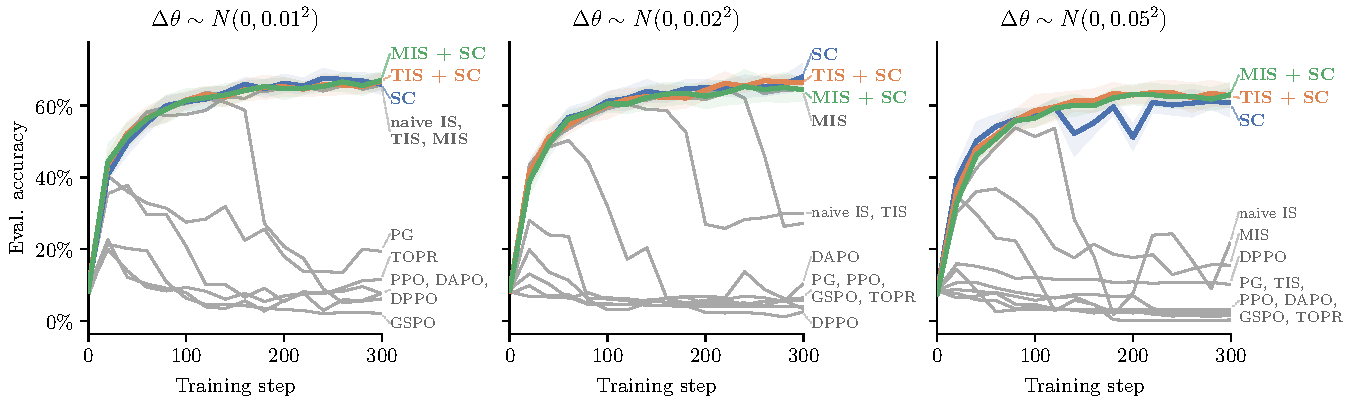
\includegraphics[width=\linewidth]{plots/06b_weight_noise.pdf}
    \caption{Qwen3-0.6B 在倒计时任务中，对采样器权重添加高斯噪声。噪声越大，越早发生坍缩。仅使用得分中心化（单独使用或与 TIS/MIS 结合）在最大噪声下仍能稳定训练。}
    \label{fig:06b_weight_noise}
\end{figure}

\subsection{量化与延迟}
\label{sec:results_quant_stale}

接下来，我们将人工权重噪声替换为两种更真实的TIM来源：量化和延迟。  
我们特意使这两种TIM来源都较为严重（\Cref{sec:results_setup}），以便在数百个训练步骤内，使用短序列长度观察不同修正方法之间的分离效果。  
在量化情景中，仅对采样器（权重、活性值和KV缓存）进行量化；而训练器使用bf16精度。  
延迟情景也故意设置得较为严重：推理引擎仅每64步更新一次，而非最大延迟为64步。  
实际上，更理想的做法是尽可能频繁地更新推理引擎（\citep{pipelineRL}），并为采样器和训练器采用相同的量化方案（\citep{jet_rl}）。

在量化采样情景（\Cref{fig:06b_quant_stale}）中，我们观察到与 \Cref{fig:06b_weight_noise} 类似的结果——仅使用得分中心化，或将其与 TIS / MIS 结合使用时表现最佳。然而，在延迟情景下，将得分中心化与 TIS / MIS 结合使用的表现最佳，优于原始的得分中心化方法。我们认为这是由于得分中心化衡量的是采样器而非训练器下的协方差 \parenCref{eq:sc_bias}：TIS 部分修正了采样分布，而得分中心化则消除了剩余的漂移。因此，当训练器在同步之间可能远离采样器时，我们建议将得分中心化与重要性采样校正结合使用。PPO 和 DAPO 在延迟情况下仍能维持性能，但在量化和权重噪声下会崩溃。这与它们的裁剪机制设计用于处理策略移动产生的比率一致：延迟会产生此类比率，而数值误差则不会。

\begin{figure}[H]
    \centering
    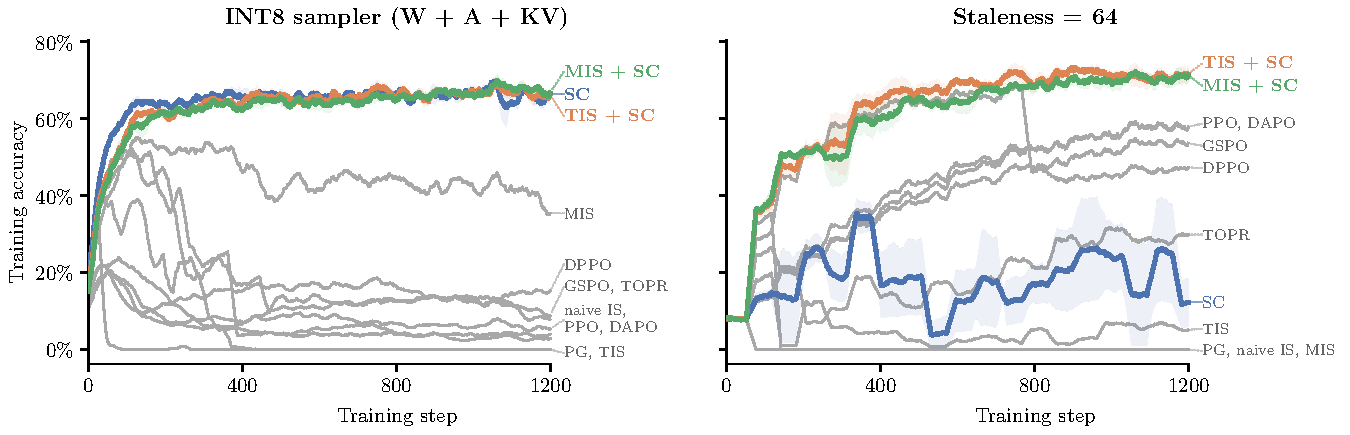
\includegraphics[width=\linewidth]{plots/06b_quant_stale.pdf}
    \caption{Qwen3-0.6B在倒计时任务中，左侧使用int8采样器，右侧使用每64步更新一次的采样器。在量化条件下，仅采用得分中心化和组合方法表现最佳；在过时性条件下，结合TIS/MIS的得分中心化组合方法占据主导地位。}
    \label{fig:06b_quant_stale}
\end{figure}

\subsection{缩放至300亿}
\label{sec:results_30b}

最后，我们通过在 INTELLECT-2 数学数据集上对 Qwen3-30B-A3B-Base 进行训练，并在采样器量化三个不同级别（\Cref{fig:30b_math}）下验证了我们的结果在更大规模下的有效性。由于 Qwen3-30B-A3B 是一个专家混合模型，采样器与训练器也可能在专家路由上产生分歧；我们未重放路由器索引，尽管在实际应用中这样做会更优 \citep{r3}。使用 FP8 采样器时，即使未经校正的策略梯度也能稳定训练，达到 $58\%$ 的训练准确率。当 KV 缓存被量化为 FP4 后，策略梯度在 200 步内崩溃，而 MIS 在训练后期才崩溃，而得分中心化（$52\%$）和 TIS（$51\%$）则保持稳定。使用 INT8 采样器和 INT4 KV 缓存时，得分中心化达到 $30\%$，TIS 达到 $12\%$，而其他所有方法均低于 $5\%$。

